\documentclass[conference]{IEEEtran}

\usepackage[latin1]{inputenc}

\usepackage{algorithm}
\usepackage{algorithmic}
	
\usepackage{amsmath}
\usepackage{amsfonts}
\usepackage{amssymb}

\usepackage{graphics}
\usepackage{graphicx}

\usepackage{caption}
\usepackage{subcaption} 

\renewcommand{\L}{\mathcal{L}}
\newcommand{\argmax}{\operatornamewithlimits{argmax}}

\author{
    \IEEEauthorblockN{Jonathan Grizou\IEEEauthorrefmark{1}, I\~naki Iturrate\IEEEauthorrefmark{2}, Luis Montesano\IEEEauthorrefmark{2}, Manuel Lopes\IEEEauthorrefmark{1}, Pierre-Yves Oudeyer\IEEEauthorrefmark{1}}
    \IEEEauthorblockA{\IEEEauthorrefmark{1} INRIA Bordeaux Sud-Ouest, France
    \\\{jonathan.grizou, manuel.lopes, pierre-yves.oudeyer\}@inria.fr}
    \IEEEauthorblockA{\IEEEauthorrefmark{2}Departamento de Inform\'atica e Ingenier\'ia de Sistemas (DIIS), Universidad de Zaragoza, Spain
    \\\{iturrate, montesano\}@unizar.es}
}

\title{\LARGE \bf Interactive Task Estimation From Unlabelled Teaching Signals}

%CHEAT CODES
\renewcommand{\baselinestretch}{.99}
\renewcommand{\textfloatsep}{0.5ex}

\begin{document}
\maketitle

\section{Introduction}

At home, workplaces or schools, an increasing amount of intelligent robotic systems are starting to be able to help us in our daily life (windows or vacuum cleaners, self-driving cars) \cite{gates2007robot} and in flexible manufacturing systems \cite{baxter}. A key feature in these new domains is the close interaction between people and robots. In particular, such robotic systems need to be teachable by non-technical users, i.e. \textbf{programmable for new tasks in novel environments} through \textbf{intuitive, flexible and personalized interactions}. Specifically, the challenge we address in this work is how a robot learning a new task can be instructed by a human using its own preferred teaching signals, where the mapping between these signals and their meaning is unknown to the robot. For example, different users may use different languages, words, interjections, gestures or even brain signals to mean ``good'' or ``bad''. 

While research on robot learning from human interaction has flourished in the last ten years \cite{Argall09lfdsurvey}, most work has focused on how to extract statistical \textit{task models} from human teachers following a fixed pre-defined teaching protocol. Thus, a usual assumption is that the learner and the teacher share a mutual understanding of the meaning of each others' signals. The question of how a robot can learn to interpret personalized and potentially noisy teaching signals, i.e.\ learn \textit{instruction models}, has been much less explored. In a preliminary work \cite{macl11simul}, we presented a computational approach addressing this problem by considering a finite space of teaching signals in simulation while bootstrapping the system with known symbols. Later \cite{grizou2013}, we released the need for bootstrapping and allow the teacher to use any kind of signal that can be represented as a fixed length feature vector, which is better suited for Human-Robot Interaction (HRI) scenario. 


Interestingly, a similar approach \cite{Kindermans2012a} has been developed in the Brain Computer Interfaces (BCI) community. Brain-computer interfaces provide a communication channel between humans and machines using only brain activity. Recent works have shown that it is possible to decode information related to human error processing, namely the error-related potentials \cite{FerrezErrores} appearing for instance when the device action does not match the user's expectations. This potential has been used as feedback information to solve sequential tasks \cite{chavarriaga2010learning}\cite{iturrate2010robot}. In practice, BCI solves the meaning problem using an open-loop calibration procedure to train a decoder in a supervised manner. 


In this abstract, we address the problem of removing the need for calibration. We propose an algorithm that simultaneously calibrates the feedback decoder and executes in closed loop a sequential task only known by the user. Our method exploits task constraints, namely optimal policies, to hallucinate the meaning of the teaching signals and select the task with the lowest expected error. We report results from a HRI scenario and a BCI online experiments. The results show that the proposed method is able to learn good feedback models while solving the task efficiently without any calibration.

In next section, we will provide an intuition on how the algorithm works without providing mathematical details. Then results from real world experiments will be briefly described, followed by the conclusion.

\section{Intuition}

In the kind of scenario we study here the user does not actively deliver commands to the robot, but only delivers feedback about actions performed by the robot. The system needs to actively execute actions to solve the tasks which implies learning the signal-to-meaning association. This control can be exemplified for a reaching task, where the user wants to reach a target position unknown by the system. The agent performs several discrete actions (e.g.\ moving left or right), and learns from the unlabelled feedback signals given by the user.

Our method exploits task constraints, namely optimal policies, to label the feedback signals according to each possible task. For each hypothesis, it is then possible to train a decoder and to compute its expected classification rate. Since the right task will assign the right labels to the signals, the expected classification rate is a good measure to identify the user's intended task. 

\begin{figure}[!h]%
\centering
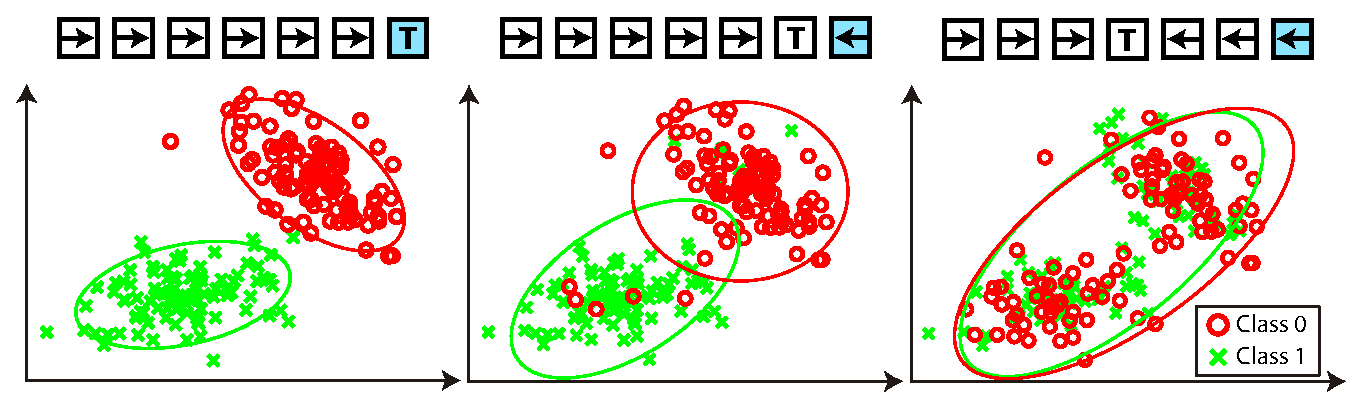
\includegraphics[width=0.85\columnwidth]{images/real_vs_fake}
\caption{Task labels for a 1-D grid world. While for the correct target the distributions shows a large separability (Left), the overlaps increases as the believed target moves away from the real one (Middle, Right). }
\label{fig:GM}
\end{figure}

The main idea is depicted in Fig~\ref{fig:GM} for a toy 1D example. The user wants the device to reach the right-most state. However, neither the target nor the feedback labels are known. The feedback signals are generated as a response to the execution of an action in a state according to the true unknown task the user wants to solve.  For instance, binary feedback signals as the ones described above simply encode whether the action executed is correct or incorrect according to the user.  The key point is that  these signals are generated from an underlying model that for binary signals has two different classes. Given sufficient feedback signals, it is possible to build the underlying distributions for each possible target. Only the right task will provide the right meanings (or labels) to each of the feedback signals (Fig.~\ref{fig:GM}~Left), while the other tasks will gradually mix both classes as the task gradually differs more to the original task (Fig.~\ref{fig:GM}~Middle-Right).

\section{Results}

\subsection{BCI Control with Human Subjects} 
We consider a 5x5 grid world, where an agent can perform five actions: move up, down, left, right, or stay. The user goal is to teach the agent to reach one of the $25$ discrete positions. During operation, the users had to assess the agent actions as good or bad, obtaining this way EEG potentials associated to correct or erroneous actions. 

The experiments were conducted with four subjects, each performing $5$ runs of learning from scratch how to reach a target (chosen randomly). The probability of the correct task is shown in Fig~\ref{fig:online_results}. All the subjects were able to identify the correct task in less than 150 steps.

\begin{figure}[!h]
	\centering
		\begin{subfigure}[t]{0.49\columnwidth}
			\centering
   			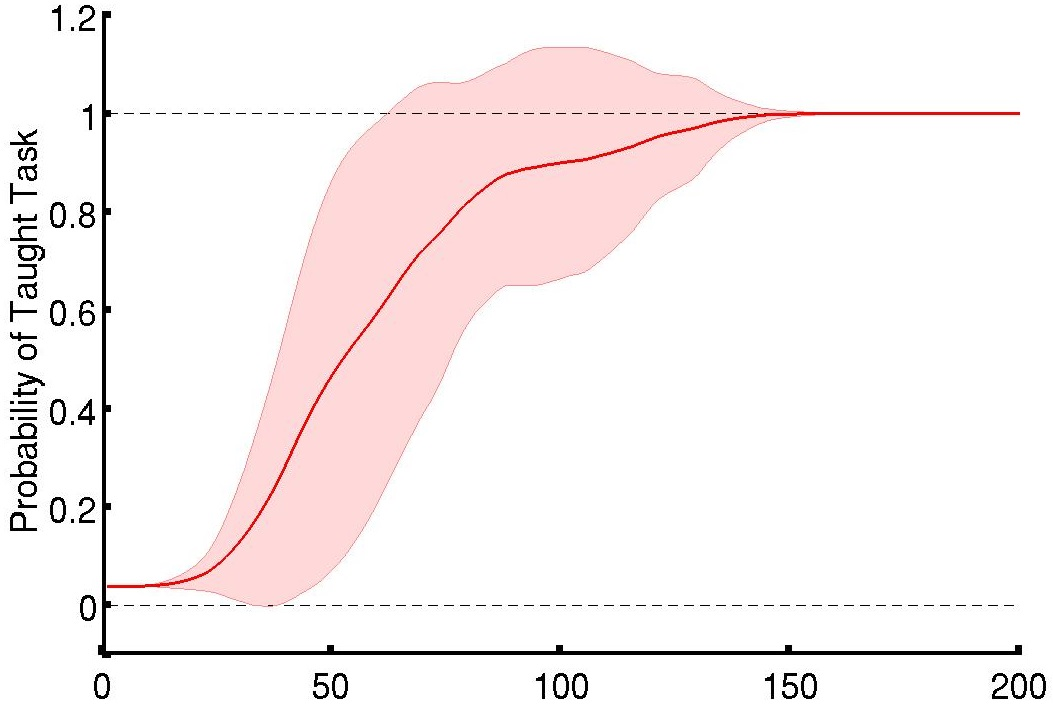
\includegraphics[width=\columnwidth]{images/Avg_evo_likelihood}
   			\caption{} 
			\label{fig:avg_evo_real}
		\end{subfigure}
		\begin{subfigure}[t]{0.49\columnwidth}
			\centering
   			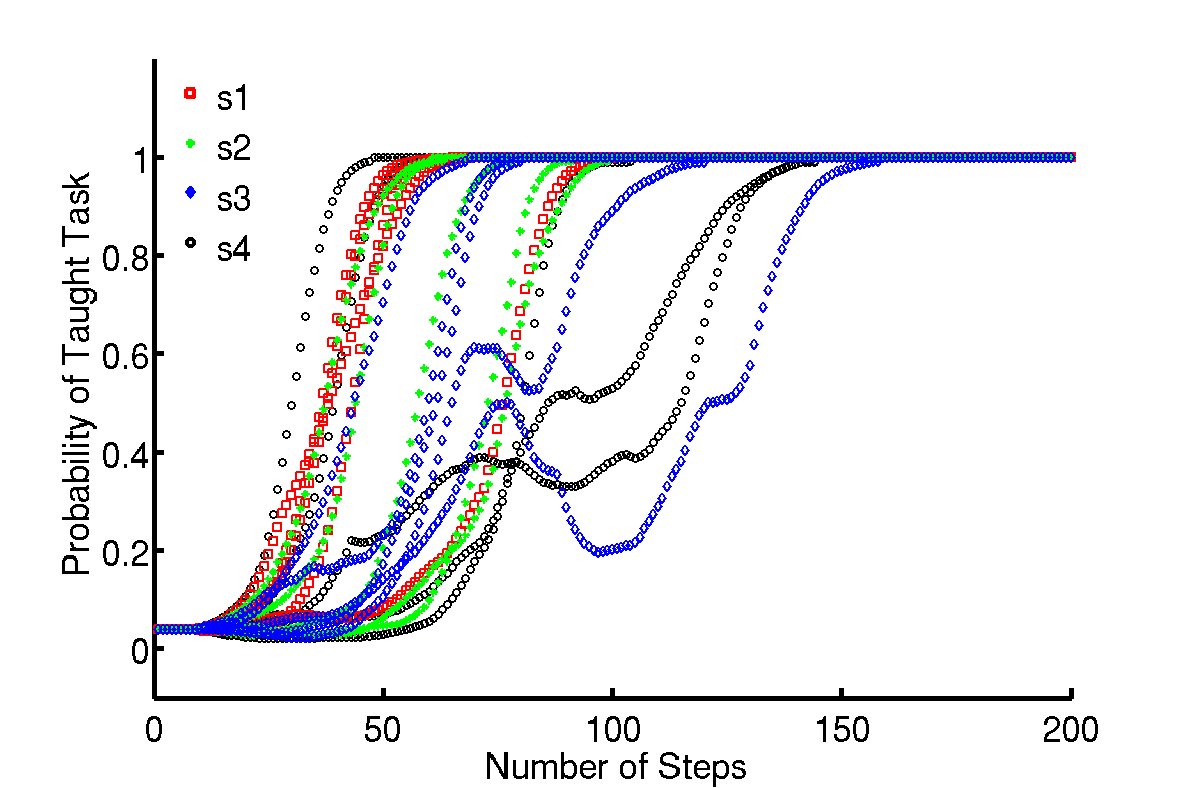
\includegraphics[width=\columnwidth]{images/Evo_likelihood}
   			\caption{} 
			\label{fig:subject_evo_real}
		\end{subfigure}
		
	\caption{\label{fig:online_results} Online experiments. Evolution of the probability of the taught task a) averaged for all subjects and, b) for each subject and run.} 
\end{figure}


\subsection{A HRI Pick and Place scenario}

We construct a small size pick-and-place task with a real robot that has 4 actions available: \textit{rotate left}, \textit{rotate right}, \textit{grasp cube} and \textit{release cube}. This robot is going to be programmed using natural speech with words a priori unknown to the robot. The teacher is facing the robot and chooses a specific arrangement of cube it wants the robot to build. It then decides one word to use as positive feedback and one as negative feedback and starts teaching the robot. Once the robot has understood the first task, we can freeze the corresponding classifier and start learning a new task, but this time the signal to meaning mapping is known.

\begin{figure}[!htbp]
	\centering
		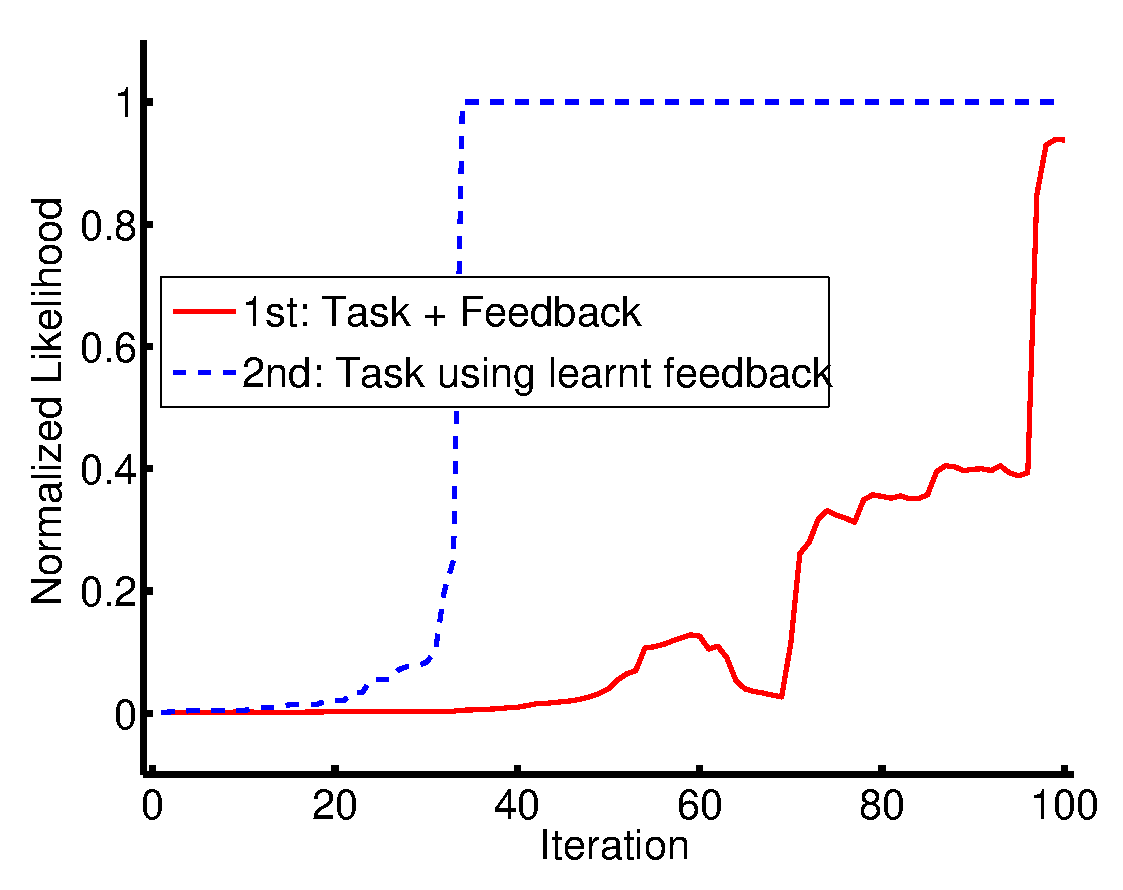
\includegraphics[width=0.5\columnwidth]{images/real}
	\caption{Evolution of the probability of the taught task. 1) The robot learns a task from unlabelled speech feedback. 2) By freezing the classifier corresponding to the best task estimate, the user teaches the robot a new task faster.}
	\label{Real}
\end{figure}

Fig.~\ref{Real} shows results from this setting. In the first run it takes about 100 iterations for the robot to learn the task. Whereas in the second run, when reusing knowledge from the first one, the robot is able to learn a new task faster, in about 30 iterations, meaning that it has well found the two clusters in our feature space as well as the mapping to their corresponding meanings.



\section{Conclusion}

We introduced a novel method for learning sequential tasks with feedback signals that do not require any calibration process. As a by-product, the method provides an unsupervised way to train a decoder while keeping the system operational and solving the unknown task. 
%
The intuition for our method is that the classification of the brain signals is easier when they are interpreted according to the target desired by the user. The method thus relies on finding which pair of decoder-target has the smaller expected prediction error in the brain signals. From another perspective, our system is able to reuse knowledge acquired from a first experiment as a source of known information for learning a new task.

\section*{Acknowledgements}
The authors from INRIA are with the Flowers Team, a INRIA / ENSTA-Paristech joint-lab. The research reported was (partially) supported by INRIA, Conseil R\'egional d'Aquitaine and the ERC grant EXPLORERS 24007.


\bibliographystyle{IEEEtran}
\bibliography{bib}

\end{document}
